
\begin{frame}{Czym jest mapa kosztów}
	\begin{itemize}
		\item mapa - informacje które punkty w przestrzeni są zajęte, ewentualnie informacje o ich identyfikacji
		\item mapa kosztów - każdy punkt w przestrzeni ma przypisaną pewną wartość (binarnie lub z większym przedziałem), wykorzystywana w algorytmach wyszukiwania ścieżki
		\item przez dodawanie wartości pośrednich można sprawić by algorytm unikał nieporządanych miejsc jak pobliże ścian czy śliska nawierzchnia
	\end{itemize}
\end{frame}

\begin{frame}{Mapa i mapa kosztów}
\begin{columns}
		\begin{column}{0.5\textwidth}
			\begin{center}
				MAPA
				\begin{figure}
					\centering
					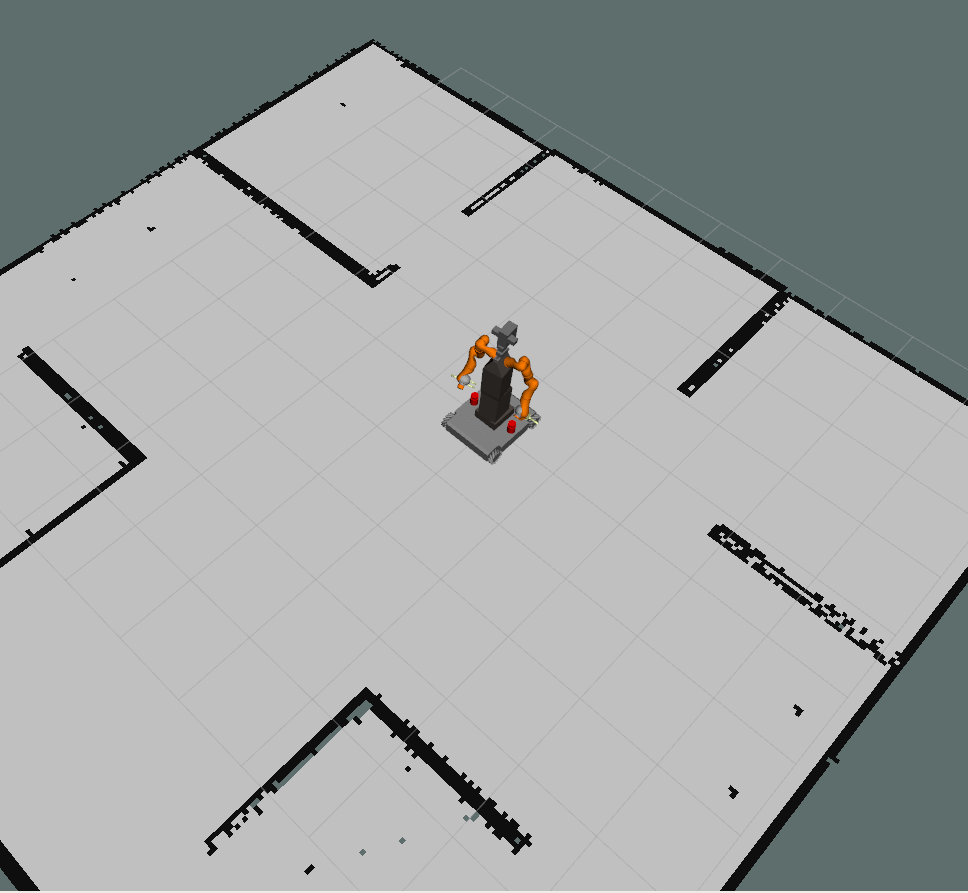
\includegraphics[height=0.55\textheight]{img/mapa_2d.png}
					\caption{dwuwymiarowa mapa środowiska}
				\end{figure}
			\end{center}
		\end{column}
		\begin{column}{0.5\textwidth}  %%<--- here
			\begin{center}
				MAPA KOSZTÓW
				\begin{figure}
					\centering
					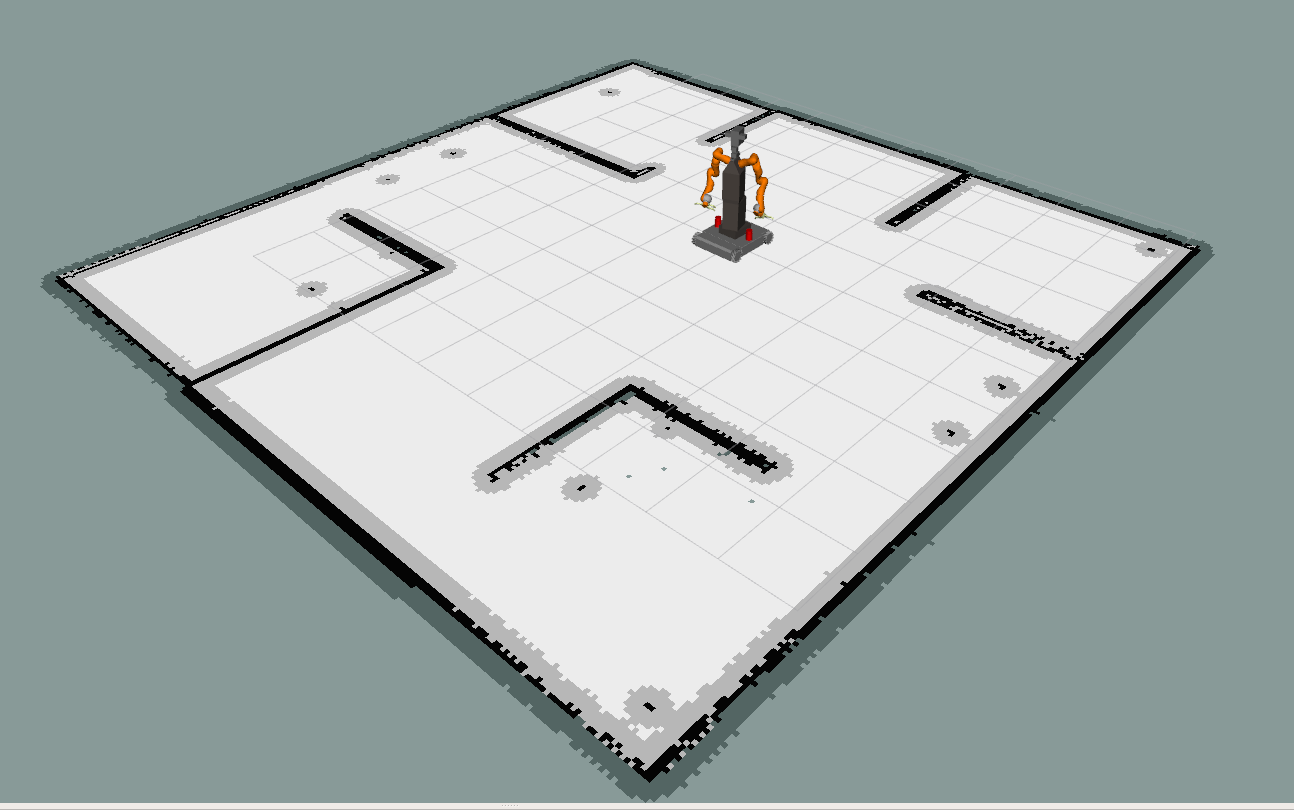
\includegraphics[height=0.55\textheight]{img/costmapa.png}
					\caption{jednowarstwowa mapa kosztów środowiska na podstawie mapy 2d}
				\end{figure}
			\end{center}
		\end{column}
	\end{columns}
\end{frame}

\begin{frame}
{Wielowarstwowe mapy kosztów}
\begin{columns}
		\begin{column}{0.5\textwidth}
			\begin{itemize}
				\item pozwalają na zobrazowanie kosztu poruszania w większej ilości kontekstów (ruch prawostronny, omijanie przestrzeni publicznej)
				\item możliwość wykrywania przeszkód na kilku poziomach (przykładowo wykrycie blatu stołu)
				\item możliwość wykorzystania chmury punktów z Kinecta do stworzenia mapy kosztów przez zrzutowanie wszystkich punktów na płaszczyznę
			\end{itemize}
		\end{column}
		\begin{column}{0.5\textwidth}  %%<--- here
			\begin{figure}
				\begin{center}
					\includegraphics[page={1},clip, trim=12.5cm 15cm 4cm 6cm, scale=0.6]{pdf/Layered_Costmaps_for_Context-Sensitive_Navigation-14.pdf}
					\hspace*{5pt}\hbox{\scriptsize{Źródło:\thinspace{\footnotesize{\itshape{David V. Lu, Dave Hershberger \cite{layered_costmap}}}}}}
					\caption{Przykład wielowarstwowej mapy kosztów }
				\end{center}
			\end{figure}
		\end{column}
	\end{columns}
\end{frame}

